\section{Battery basics}
\label{sec:pastwork:basics}

For the purposes of the studies explored in this dissertation, we define a battery as an electrochemical cell (often referred to as a "cell") capable of storing and providing electrical energy through the use of oxidation and reduction reactions between two electrodes surrounded by an ion-conducting electrolyte. A schematic battery is shown in Fig.~\ref{fig:echemschem}. The electrode at which reduction reactions occur is called the cathode, while the electrode where oxidation occurs is called the anode. During discharge, the cathode is referred to as the positive electrode and the anode is referred to as the negative electrode. Batteries are categorized as either primary (single-use) or secondary (rechargeable). In both, discharge occurs by connecting the battery electrodes in series with a resistive load, and in secondary batteries, charging occurs by applying a voltage or current to the battery electrodes, reversing the redox reactions that occurred during discharge, while reversing the positive/negative convention for the cathode/anode. During discharge, electrons flow from the anode through an external circuit before terminating at the cathode. The method of discharge can be controlled by drawing a constant voltage or a constant current from the cell. Once the battery voltage or current falls beneath a given threshold, the cell is considered "dead."

\begin{figure}[htb]
  \centering
    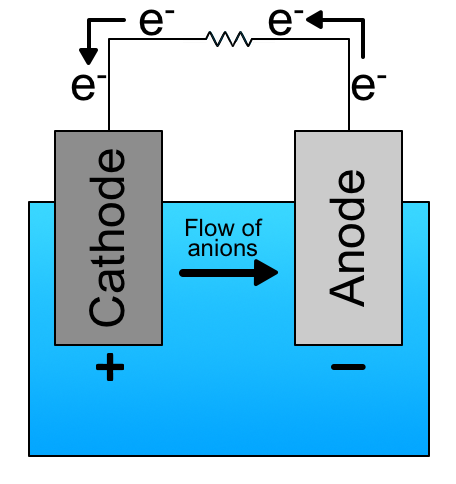
\includegraphics[width=0.5\textwidth]{ch2-pastwork/images/echemschem.png}
    \caption[Schematic of an electrochemical cell during discharge.]{Schematic of an electrochemical cell during discharge, with electrodes and flow of electrons and anions labeled.}
    \label{fig:echemschem}
\end{figure}


In battery literature, an oft-mentioned metric is the state of charge (SOC) which provides a measure of how much of the initial capacity of a battery still remains after a given amount of discharge. Typically, state of charge can be expressed as a percentage. A second, more complicated metric is the state of health (SOH). SOH (also expressed as a percentage) can be thought of as a measure of capacity fade, comparing the available total capacity for a given charge/discharge cycle to the initial total capacity. In this way, it functions like a time-resolved SOC. All batteries experience some capacity fade with use, and SOH is still a very difficult metric to measure directly. The last metric that is referenced often is the "C rate," written in the form C/2 or 2C. The "C" in this metric refers to the cell capacity in ampere-hours (Ah) or milli-ampere-hours (mAh), and the numeral refers to the inverse of the number of hours over which the capacity should be discharged. For example, C/2 would refer to a rate at which full capacity is discharged in two hours, while 2C refers to a rate at which cell capacity is discharged in 0.5 hours. Figure~\ref{fig:dischcurve} shows the difference between an ideal discharge curve, showing a constant voltage over the entire capacity of the cell, and an actual discharge curve, showing the non-idealities that come from ohmic, kinetic and mass transport limitations. Generally, the greater the discharge rate, the greater the slope of the discharge curve. A flatter discharge curve means that the voltage supplied is more constant, but this can make certain methods of state of charge estimation difficult. 

\begin{figure}[htb]
  \centering
    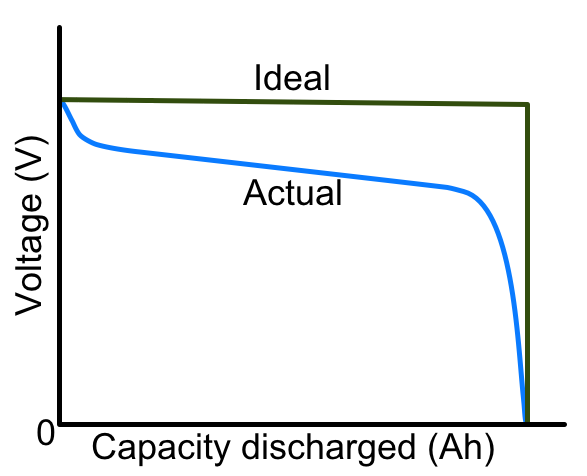
\includegraphics[width=0.5\textwidth]{ch2-pastwork/images/dischcurves.png}
    \caption[Example discharge curves.]{Example of an ideal and an actual discharge curve of a battery.}
    \label{fig:dischcurve}
\end{figure}

Many chemistries of both primary and secondary batteries exist. A common figure used to compare energy density and power density is the Ragone plot, shown for both primary and secondary batteries in Fig.~\ref{fig:ragone}.~\cite{ragone_primary,ragone_secondary} Ragone plots offer a straightforward method of narrowing down a battery chemistry based on energy or power needs. Furthermore, a cell's open circuit voltage can be estimated from a list of standard reduction potentials, which can further help to match a chemistry to an application.

\begin{figure}[htb]
  \centering
    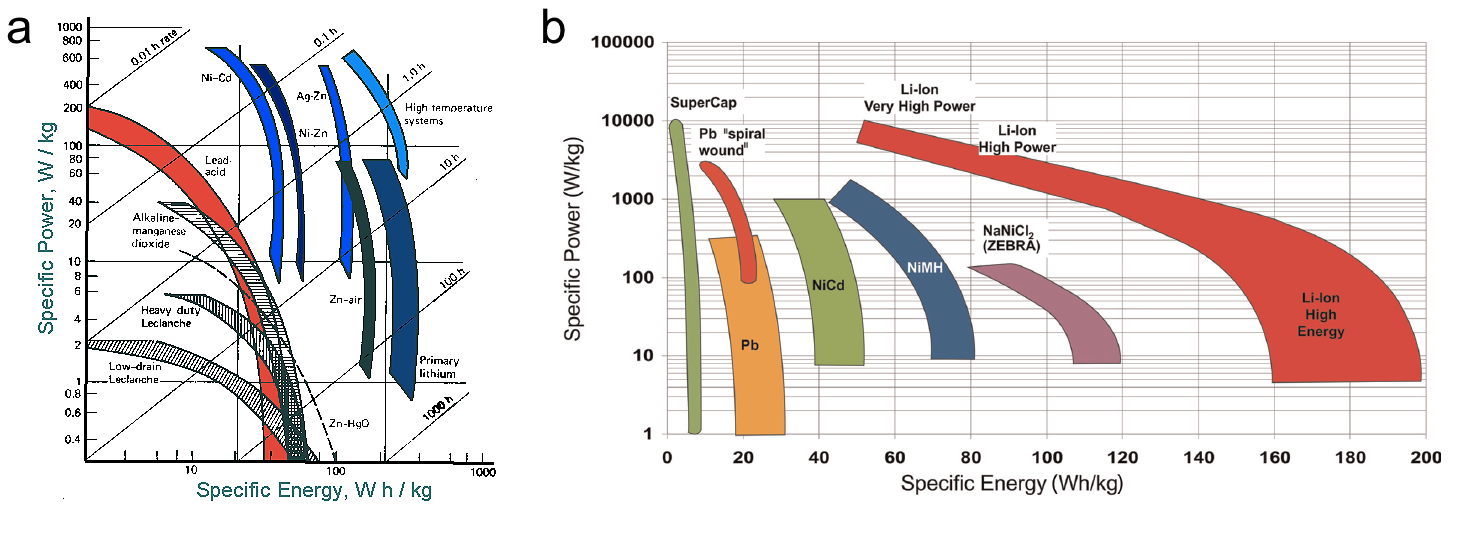
\includegraphics[width=\textwidth]{ch2-pastwork/images/ragone.png}
    \caption[Ragone plot of primary and secondary batteries.]{Ragone plot for \textbf{(a)} primary batteries, and \textbf{(b)} secondary batteries.}
    \label{fig:ragone}
\end{figure}

\subsection{Alkaline batteries}

The mainstay of the primary battery market is the alkaline battery, named for its use of KOH as an electrolyte. The chemistry and form factor have been popular for over 50 years because of the low cost of the source material (Zn) and the  bobbin cell design.~\cite{karl_patent} The bobbin cell construction is demonstrated in Fig.~\ref{fig:aaschem} along with the typical method of cell assembly is detailed in Fig.~\ref{fig:cellassembly}.~\cite{fujitsu} 

\begin{figure}[htb]
  \centering
    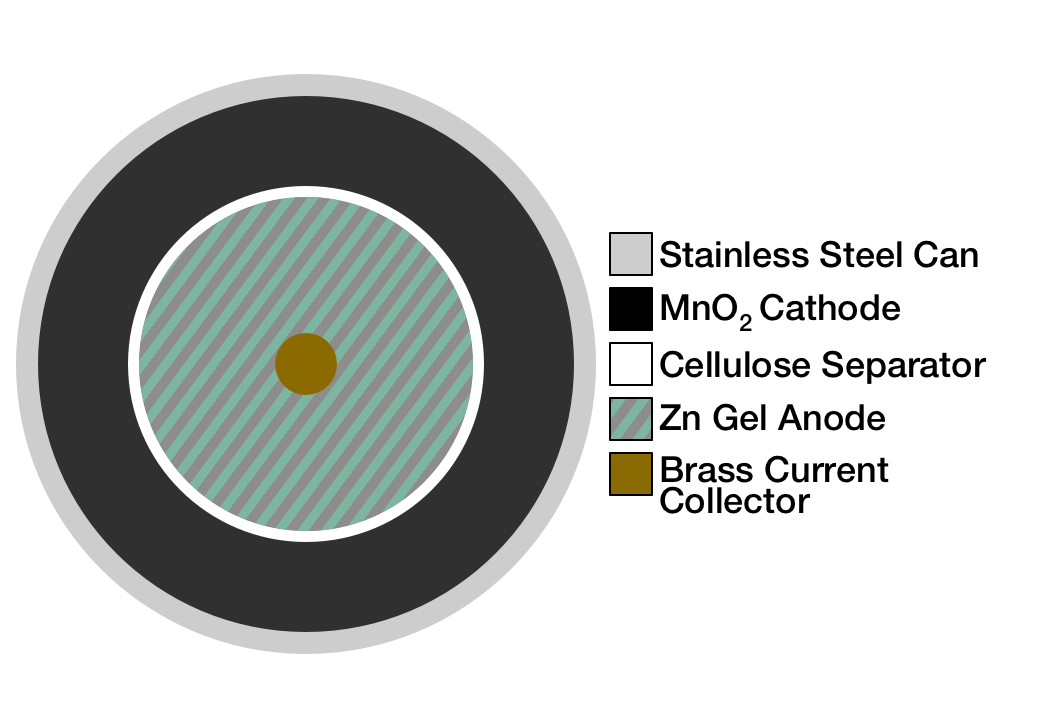
\includegraphics[width=0.60\textwidth]{ch3-dbb/Images/aaschem.png}
    \caption[Schematic of construction of an alkaline AA battery.]{Schematic of construction of an alkaline AA battery. Components are labeled according to the legend.}
    \label{fig:aaschem}
\end{figure}

\begin{figure}[htb]
  \centering
    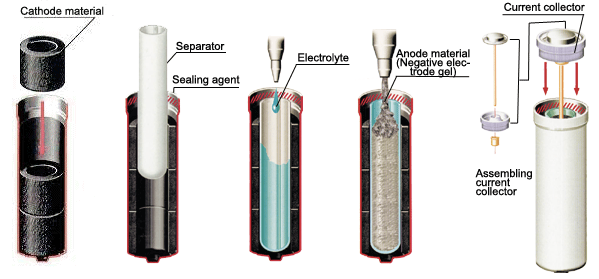
\includegraphics[width=\textwidth]{ch2-pastwork/images/cellassembly.png}
    \caption[Assembly process of alkaline AA batteries.]{Assembly process of alkaline AA batteries.}
    \label{fig:cellassembly}
\end{figure}

Each cell comprises a stainless steel can containing concentric layers of a \ce{MnO_2} cathode, a cellulose separator, a Zn gel anode containing KOH and a gelling agent, and a central brass current collecting pin. It is available in a number of sizes, with the most common sizes being the AA, AAA, C and D cell specifications, with a nominal voltage of 1.5 V.~\cite{linden} As the cell is discharged, the Zn anode is oxidized to ZnO, while the \ce{MnO_2} cathode is reduced through proton insertion into a variety of discharge products ranging from \ce{MnOOH} to \ce{ZnMn2O4}, depending on discharge rate.~\cite{Gallaway2015-xy}


\subsection{Lithium-ion batteries}

If alkaline batteries are the mainstays of the primary battery market, then lithium-ion batteries (LIBs) are almost certainly the equivalent mainstay of the secondary battery market. Popularized by consumer electronics and electric vehicles, LIBs offer some of the highest energy densities of current electrochemical storage methods.~\cite{linden}. A wide range of chemistries exist, and most LIBs have a wound construction in which layers of anode, polymeric separator, cathode, and current collector films are assembled in a stack and then wound to produce a final geometry, as demonstrated in Fig.~\ref{fig:libgeom}. Cells can be wound in a prismatic fashion to produce ``pouch" cells that have a rectangular cross section, or in a cylindrical fashion to produce ``jelly roll" cells. The former is most commonly used in portable electronic devices, while the latter has found use in laptop computers and electric vehicles such as the Tesla Model S.

\begin{figure}[htb]
  \centering
    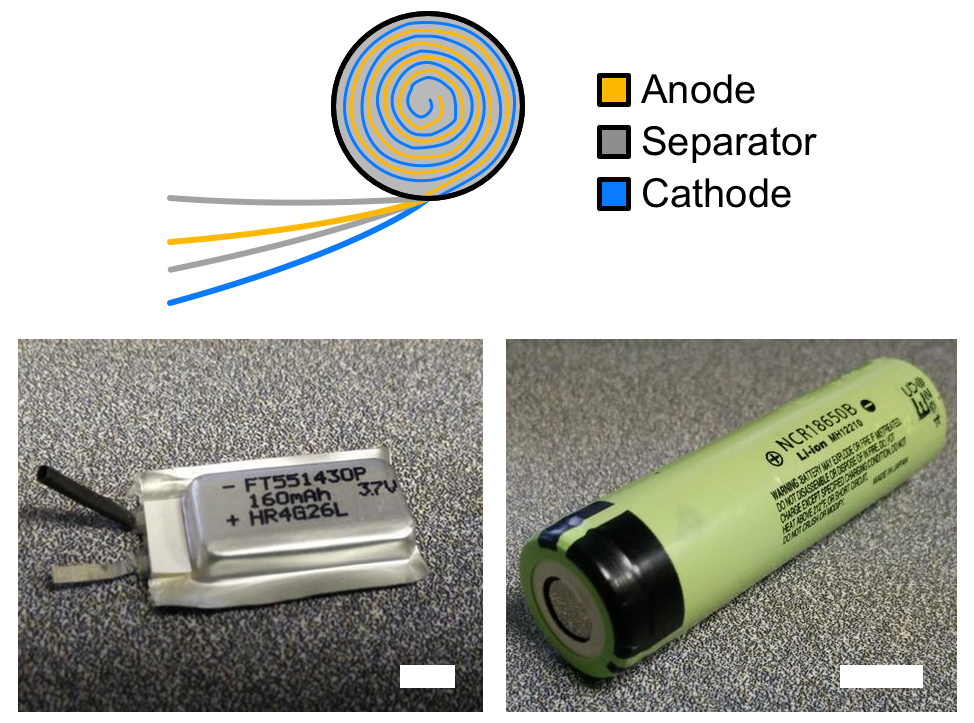
\includegraphics[width=0.8\textwidth]{ch2-pastwork/images/libgeom.png}
    \caption[Lithium-ion battery geometries.]{\textbf{(Top)} Schematic of a wound lithium-ion battery. \textbf{(Left)} \ce{LiCoO2} pouch cell.\textbf{(Right)} \ce{Li(NiCoAl)O2} ``jelly roll" cell.}
    \label{fig:libgeom}
\end{figure}

LIBs typically operate between 2.5 V and 4.2 V, with an average voltage of 3.7 V.~\cite{linden} Charging and discharging occur via a reversible intercalation process: during charge, lithium ions intercalate within the layers of the anode material, while during discharge, lithium ions intercalate into the cathode material while donating electrons to an external load. The typical anode material used in LIBs is graphite, owing to its layered structure. A considerable number of cathode chemistries exist, but this dissertation discusses only two of them: \ce{LiCoO2} and \ce{Li(NiCoAl)O2}. Both are layered oxides, but \ce{LiCoO2} has a slightly higher voltage vs. Li (3.9 V) while \ce{Li(NiCoAl)O2} has a higher specific capacity (200 mAh/g).~\cite{linden} 


